\chapter[Идентификация нелинейных стохастических систем второго типа]{%
  Идентификация нелинейных стохастических систем второго типа
}

\section{Математическая модель идентифицируемой системы}

Для обеспечения наглядности сравнения рассматривался случай идентификации скалярной системы:
\begin{equation}
  \label{eq:nonlinear_model_scalar}
  \begin{aligned}
  h &= \psi(\theta, \xi), \\
  x &= \xi + \varepsilon_x, \\
  y &= h + \varepsilon_y,
  \end{aligned}
\end{equation}
где \( \xi, h \) "--- фактические значения входной и выходной переменной, \par
\( \psi \) "--- скалярно-векторная функция регрессии, \par
\( \theta = (\theta_1, \theta_2, \dotsc, \theta_m) \) "--- вектор фактических значений параметров объекта, \par
\( x, y \) "--- измеренные значения входной и выходной переменной, \par
\( \varepsilon_x, \varepsilon_y \) "--- независимые ошибки измерений значений входной и
выходной переменной, распределенные по нормальному закону:
\(
\varepsilon_x = N(0, \sigma_{\varepsilon_x}),
\varepsilon_y = N(0, \sigma_{\varepsilon_y})
\).

Данная модель использовалась для генерации наблюдений входа и выхода системы,
на основании которых были получены оценки её параметров методами на основе
классического и симметричного критериев аппроксимации.
Значения \( \xi_i \) выбирались из равномерного в \( [0, 10] \) распределения.
Для получения каждой оценки \( \hat{\theta} \) использовались результаты
ста наблюдений \( ( x_i, y_i ), i = \overline{1, n}, n = 100 \).

\section{Алгоритмы методов идентификации}

\subsection{Нелинейный метод наименьших квадратов}

Один из подходов к оценке параметров системы~\eqref{eq:nonlinear_model_scalar} состоит в следующем.
Можно <<закрыть глаза>> на существование ошибок измерений
входной переменной, то есть считать, что \( \varepsilon_x = 0 \),
и вместо данной модели рассматривать модель
\begin{equation}
  \label{eq:nonlinear_model_lse}
  \begin{aligned}
  x &= \psi(\theta, \xi), \\
  y &= x + \varepsilon_y.
  \end{aligned}
\end{equation}

Тогда оценка вектора параметров объекта определяется выражением~\cite{mukha_2009}
\begin{equation}
  \label{eq:nonlinear_lse}
  \hat{\theta}_{\text{НМНК}} =
  \theta_0 + (Q^T R^{-1}_{\Xi} Q)^{-1} Q^T R^{-1}_{\Xi} (y - \psi(\theta_0, x)),
\end{equation}
где \( \theta_0 \) --- опорная точка,
\( Q = \dfrac{\partial \psi(\theta_0, x) }{ \partial \theta_0 } \).

Эту оценку будем называть оценкой, полученной нелинейным
методом наименьших квадратов (НМНК).
В качестве опорной точки \( \theta_0 \) можно использовать значение
\( \theta_1, \dotsc, \theta_m \),
полученное в результате численного решения системы уравнений
\begin{equation}
  \label{eq:nonlinear_basic}
  (y_j - \psi( \theta, x_j )) = 0, \: j = \overline{1,m},
\end{equation}
где \( x_j, y_j \) --- опорные наблюдения входа и выхода системы соответственно.

В качестве опорных могут выступать, например:
\begin{itemize}
\item первые пары наблюдений:
  \[ (x_1, y_1), (x_2, y_2), \dotsc , (x_m, y_m); \]
\item равноотстоящие пары наблюдений:
  \[
    (x_{k}, y_{k}), (x_{2k}, y_{2k}) , \dotsc , (x_{mk}, y_{mk}), \:
    k = \lfloor \dfrac{n}{m} \rfloor;
  \]
\item крайние пары наблюдений:
  \[
    (x_{1}, y_{1}), (x_{1 + k}, y_{1 + k}) , \dotsc , (x_{n}, y_{n}), \:
    k = \lfloor \dfrac{n-1}{m-2} \rfloor;
  \]
\item усредненные наблюдения:
  \begin{gather*}
    ( \overline{x}_{k}, \overline{y}_{k} ),
    ( \overline{x}_{2k}, \overline{y}_{2k} ),
    \dotsc ,
    ( \overline{x}_{mk}, \overline{y}_{mk}), \\
    \overline{x}_{ik} = \dfrac{1}{m} \sum_{j = 1+(i-1)k}^{ik} x_j, \quad
    \overline{y}_{ik} = \dfrac{1}{m} \sum_{j = 1+(i-1)k}^{ik} y_j, \quad
    k = \lfloor \dfrac{n}{m} \rfloor.
  \end{gather*}
\end{itemize}

Для уточнения оценки, полученной по формуле~\eqref{eq:nonlinear_lse}, можно
организовать итерационную процедуру, заменяя опорную точку полученной оценкой.

\vspace{2\baselineskip}
\subsection{Метод рядов Тейлора}

Применение метода рядов Тейлора (МРТ)~\cite{mukha_2000}
требует иной формулировки задачи, допускаемой формулировкой \eqref{eq:nonlinear_model_scalar}.
Следует предположить, что \( j \)-е наблюдение вектора параметров \( \theta_j \)
определяется как векторная функция показаний приборов:
\begin{equation}
  \label{eq:nonlinear_mrt_phi}
  \theta_j = \phi( \overline{z}_{j} ), \: j = \overline{1, n},
\end{equation}
где вектор
\( \overline{z}^{\text{T}}_{j} =
( \overline{x}^{\text{T}}_{j}, \overline{y}^{\text{T}}_{j}) \)
имеет нормальное распределение \( N(A_{z,j}, R_{z,j}) \)
и оцениваемый векторный параметр \( \theta \) определяется как
\( \theta = \phi(A_{z,j}), \forall i = \overline{1, n} \).
В этом случае МРТ-оценка \( \hat{\theta}_{\text{МРТ}} \) векторного параметра \( \theta \)
определяется выражением
\begin{equation}
  \label{eq:nonlinear_mrt}
  \hat{\theta}_{\text{МРТ}} =
  \Bigg( \sum^{n}_{i=1} R^{-1}_{\theta,i} \Bigg)^{-1}
  \sum^{n}_{j=1} R^{-1}_{\theta,j} \theta_j,
\end{equation}
где
\( R_{\theta,i} = G_i R_{z,i} G^T_i \),
\( G_i =
\dfrac{\partial \phi( \overline{z}_{i} ) }{ \partial \overline{z}_{i} } \).

Численное значение наблюдения \( \theta_j \)~\eqref{eq:nonlinear_mrt_phi} может определяться как
решение системы уравнений~\eqref{eq:nonlinear_basic}.


\section{Численный анализ точности оценивания параметров}

\subsection{Методика сравнения}

Было выполнено сравнение точности оценок,
полученных нелинейным методом наименьших квадратов и методом рядов Тейлора,
для функций регрессии различного вида,
в зависимости от с.~к.~о ошибок измеряемых значений
\( \sigma_{\varepsilon_x}, \sigma_{\varepsilon_y} \).

В качестве величины, характеризующей сравнительную точность оценивания параметров,
использовалась разность средних Евклидовых расстояний
между точными значениями параметров модели и их оценками, полученными
с помощью НМНК и МРТ:
\begin{equation}
  \begin{aligned}
    d &= d_{\text{НМНК}} - d_{\text{МРТ}}, \\
    d_{\text{НМНК}} &=
    \frac{1}{k} \sum_{j=1}^k
    \sqrt{\sum_{\text{i=1}}^m (\hat{\theta}_{\text{НМНК}_{ij}} - \theta_{ij})^2}, \\
    d_{\text{МРТ}} &=
    \frac{1}{k} \sum_{j=1}^k
    \sqrt{\sum_{\text{i=1}}^m (\hat{\theta}_{\text{МРТ}_{ij}} - \theta_{ij})^2}.
  \end{aligned}
  \label{eq:dst_nonlinear_param}
\end{equation}

Расчеты величины \( d \) производились в узлах сетки значений
\( \sigma_{\varepsilon_x}, \sigma_{\varepsilon_y} \) в прямоугольнике
\( [0, 2] \times [0, 2] \) с шагом 0{,}1.
В каждом узле сетки вычислялось \( k = 100 \) оценок.
Для расчтеа оценок использовались крайние опорные наблюдения.
В качестве значений НМНК-оценки \( \theta_{\text{НМНК}} \)
использованы значения, полученные на первой итерации метода.

\vspace{2\baselineskip}
\subsection{Линейная функция регрессии}

Частным случаем нелинейной модели~\eqref{eq:nonlinear_model_scalar} является линейная,
то есть такая, функция регрессии которой имеет вид \( \psi = \theta_1 + \theta_2 \xi \).

На рисунке~\ref{fig:comparison_nonlinear_linear}
представлены графики функции \( d(\sigma_{\varepsilon_x}, \sigma_{\varepsilon_y}) \)
при различных значениях параметра \( \theta_2 \).
По результатам сравнения можно заключить, что точность оценивания параметров линейных моделей
не зависят от постоянной составляющей \( \theta_1 \), и что оценки, полученные с помощью НМНК,
являются более точными во всем диапазоне величин \( \theta_2 \).

\begin{figure}[p]
  \begin{subfigure}[b]{\linewidth}
    \centering
    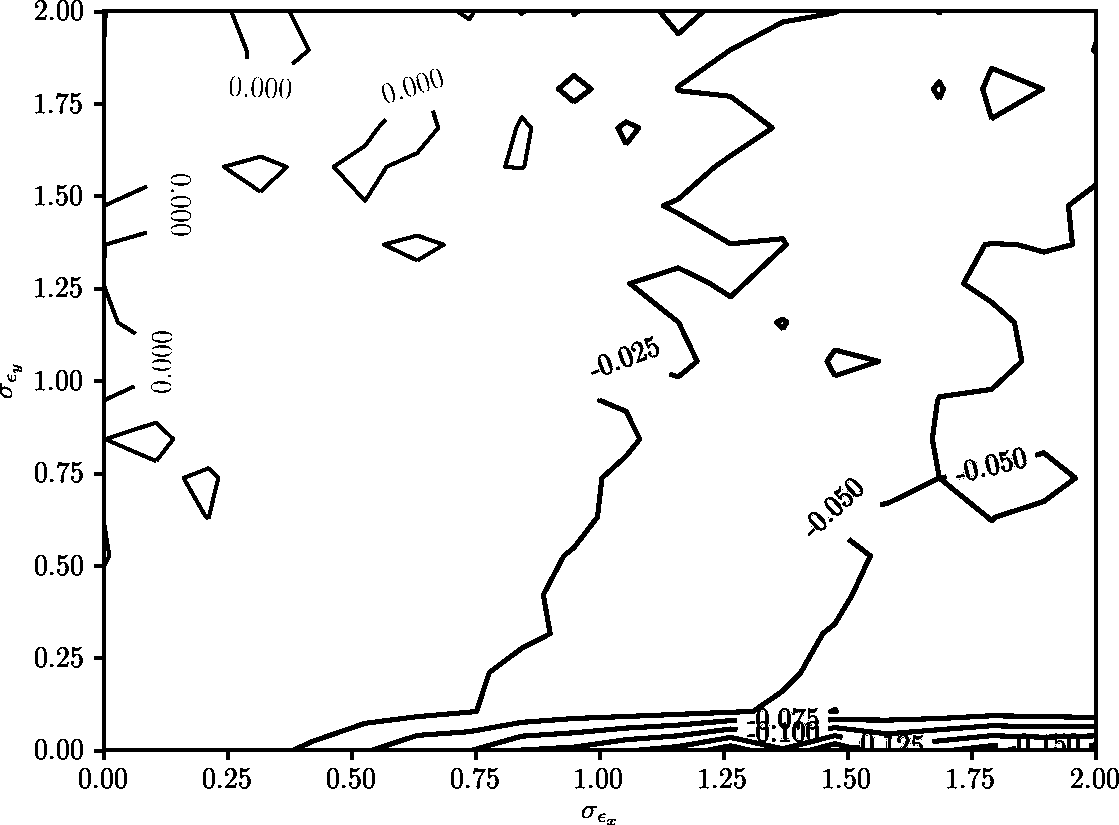
\includegraphics[width=135mm]{fig/nonlinear/linear/beta-0,2.png}
    \caption{\( \theta_2 = 0{,}2 \)}
  \end{subfigure}

  \vspace{2\baselineskip}
  \begin{subfigure}[b]{\linewidth}
    \centering
    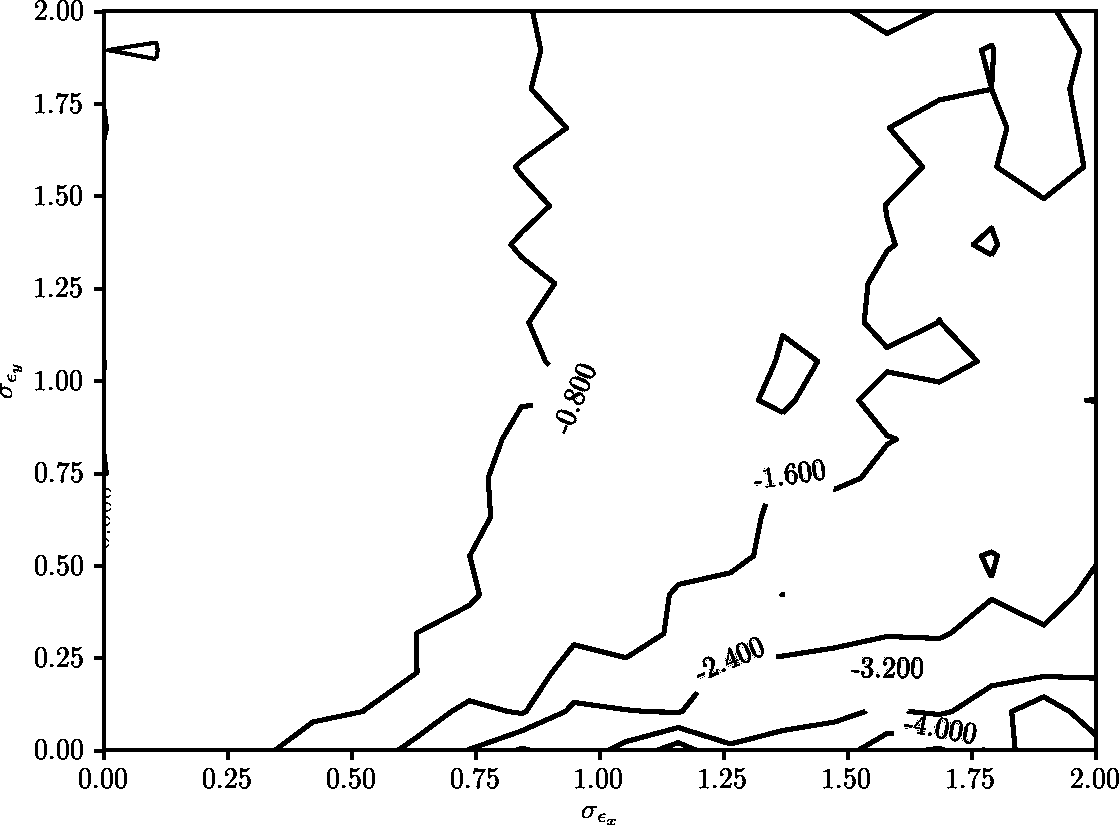
\includegraphics[width=135mm]{fig/nonlinear/linear/beta-5.png}
    \caption{\( \theta_2 = 5 \)}
  \end{subfigure}

  \vspace{\baselineskip}
  \caption{%
    Точность оценивания \\
    параметров линейной модели
  }\label{fig:comparison_nonlinear_linear}
\end{figure}

\subsection{Параболическая функция регрессии}

Параболическая функция регрессии является, пожалуй, наиболее <<популярной>> из нелинейных.
Поскольку ранее было установлено, что постоянная составляющая не влияет на точность оценивания,
рассматривалась функция вида \( \psi = \theta_1 \xi + \theta_2 \xi^2 \).

На рисунке~\ref{fig:comparison_nonlinear_quadratic_alpha-0_beta-1}
представлен график функции \( d(\sigma_{\varepsilon_x}, \sigma_{\varepsilon_y}) \)
для параболической функции регрессии при \( \theta_1 = 0, \theta_2 = 1 \).
Видно, что в данном случае МРТ-оценки параметров, являются более точными,
чем оценки, полученные с помощью НМНК.

\begin{figure}[h!]
  \centering
  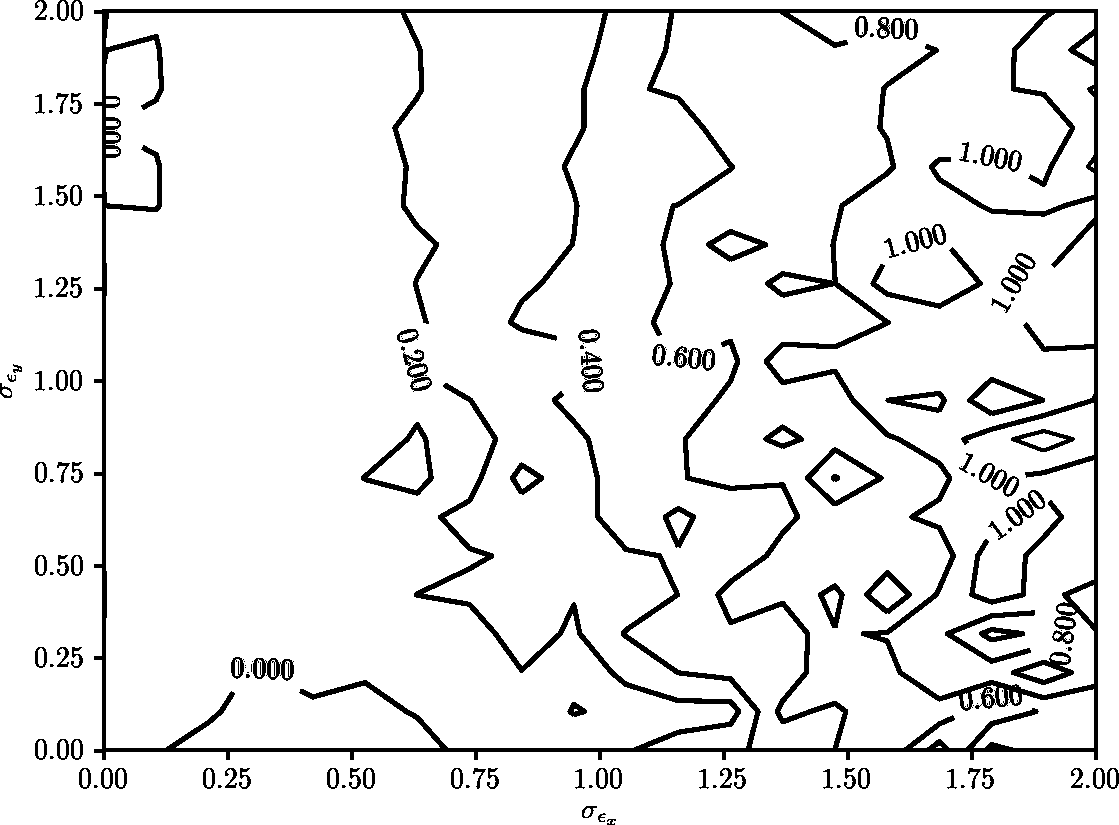
\includegraphics[width=135mm]{fig/nonlinear/quadratic/alpha-0_beta-1.png}
  \caption{
    Точность оценивания параметров \\
    параболической модели при \( \theta_1 = 0, \theta_2 = 1 \)
  }\label{fig:comparison_nonlinear_quadratic_alpha-0_beta-1}
\end{figure}

На рисунке~\ref{fig:comparison_nonlinear_quadratic_alpha-0}
представлены графики функции \( d(\sigma_{\varepsilon_x}, \sigma_{\varepsilon_y}) \)
при \( \theta_1 = 0 \). В обоих случаях МРТ-оценки оказались более точными.

\begin{figure}[p]
  \begin{subfigure}[b]{\linewidth}
    \centering
    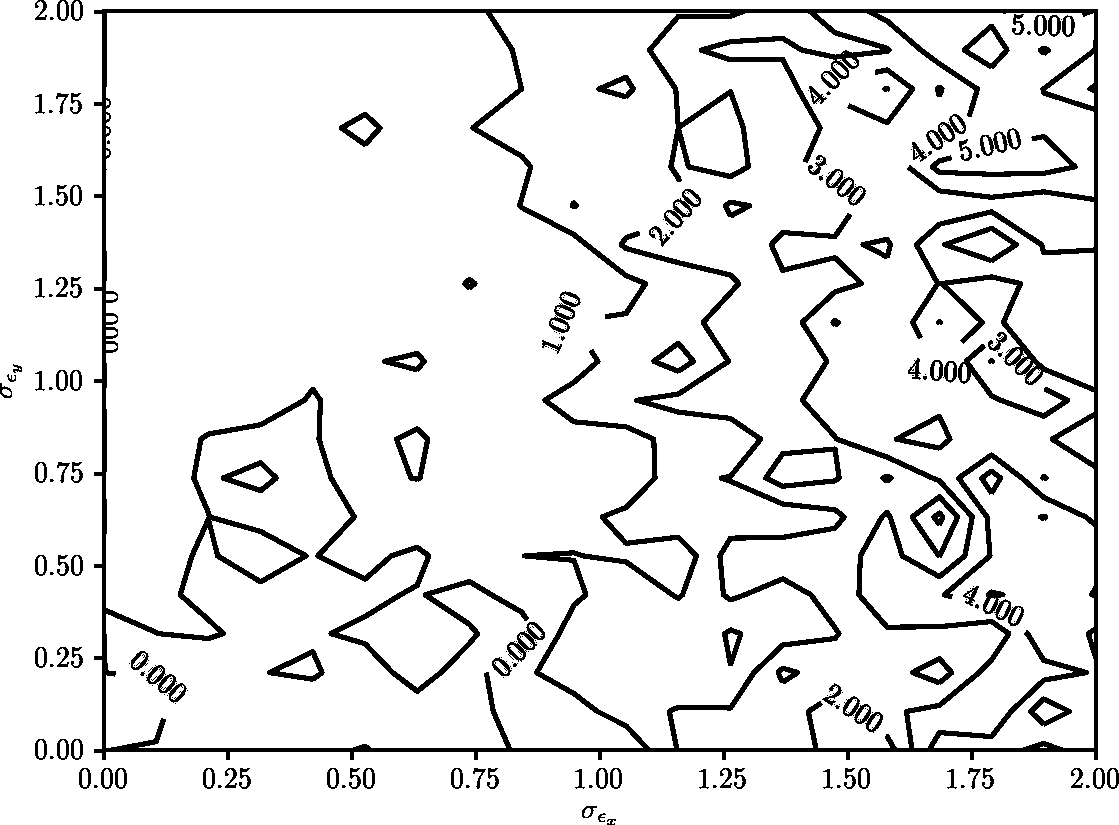
\includegraphics[width=135mm]{fig/nonlinear/quadratic/alpha-0_beta--5.png}
    \caption{\( \theta_2 = -5 \)}
  \end{subfigure}

  \vspace{2\baselineskip}
  \begin{subfigure}[b]{\linewidth}
    \centering
    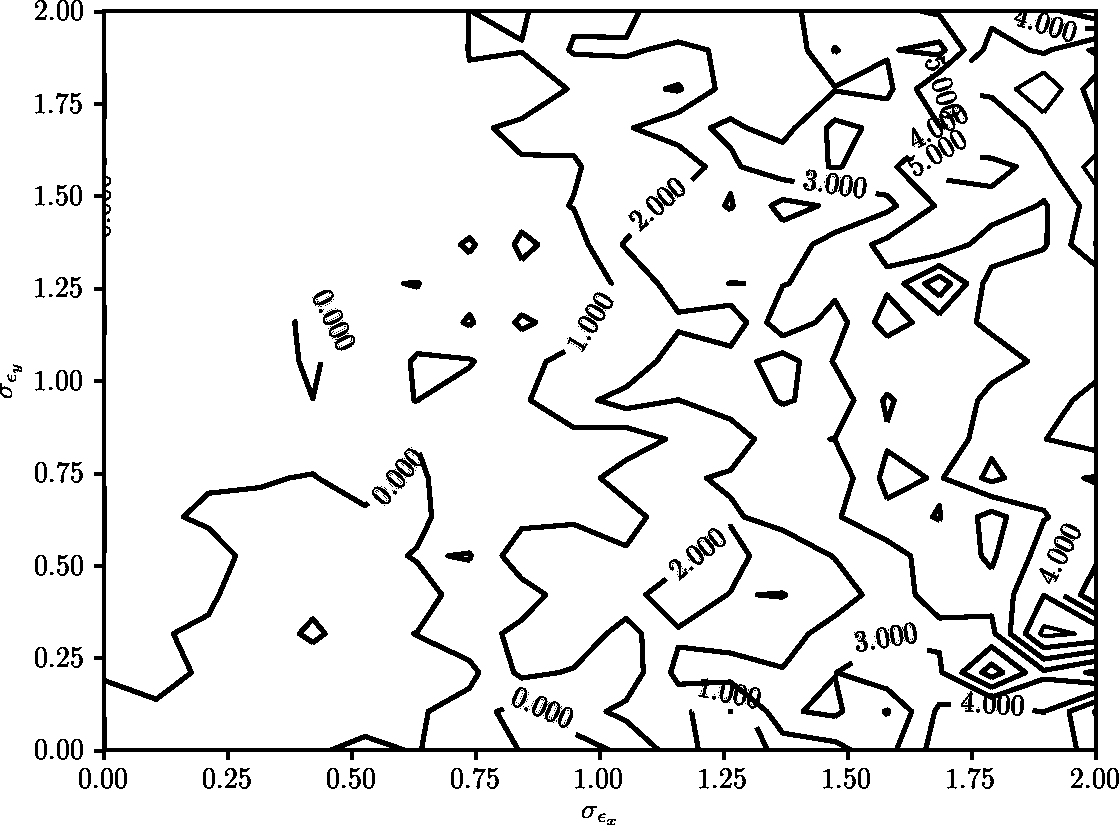
\includegraphics[width=135mm]{fig/nonlinear/quadratic/alpha-0_beta-5.png}
    \caption{\( \theta_2 = 5 \)}
  \end{subfigure}

  \vspace{\baselineskip}
    \caption{
      Точность оценивания параметров \\
      параболической модели при \( \theta_1 = 0 \)
    }\label{fig:comparison_nonlinear_quadratic_alpha-0}
\end{figure}

На рисунке~\ref{fig:comparison_nonlinear_quadratic_beta-1}
представлены графики функции \( d(\sigma_{\varepsilon_x}, \sigma_{\varepsilon_y}) \)
при \( \theta_2 = 1 \).
В первом случае (рисунок~\ref{fig:comparison_nonlinear_quadratic_alpha--5_beta-1})
МРТ-оценки оказались более точными, чем НМНК, а во втором
(рисунок~\ref{fig:comparison_nonlinear_quadratic_alpha-5_beta-1}) --- наоборот.
Это связано, по-видимому, с тем, что выражение \( -5 \xi + \xi^2 \)
обладает более ярко выраженной <<нелинейностью>>, чем \( 5 \xi + \xi^2 \).

\begin{figure}[p]
  \begin{subfigure}[b]{\linewidth}
    \centering
    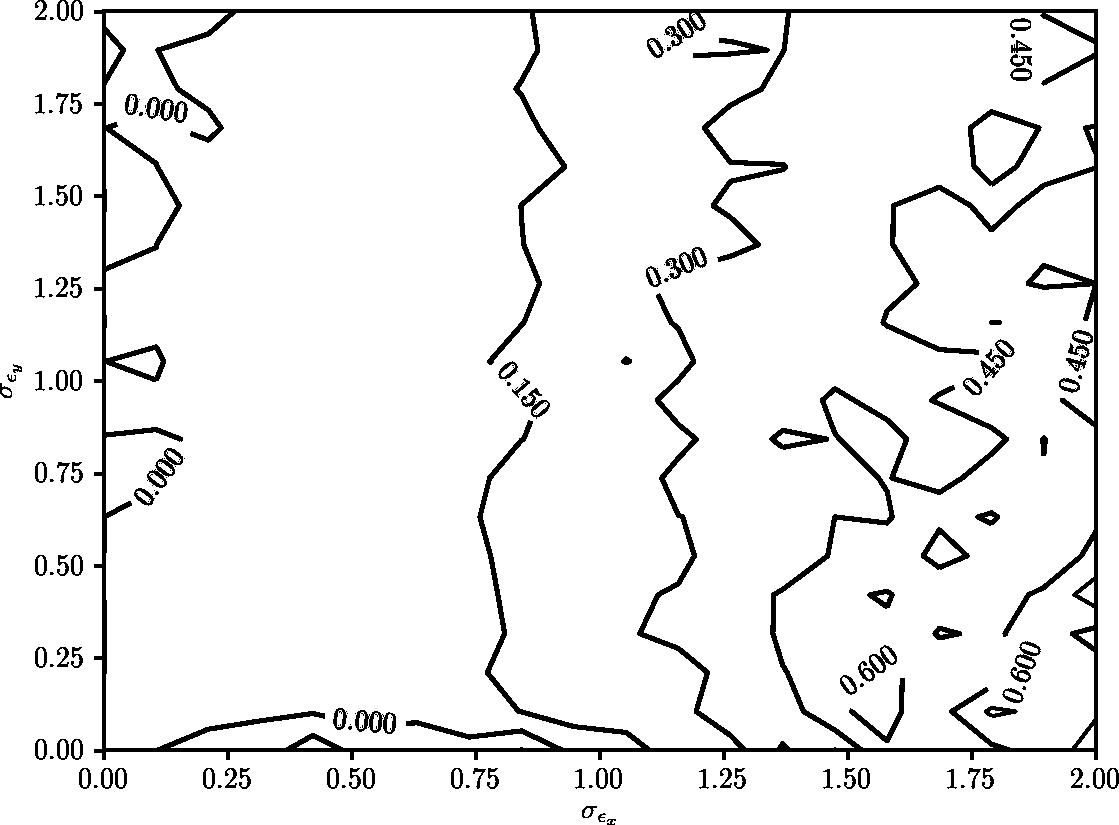
\includegraphics[width=135mm]{fig/nonlinear/quadratic/alpha--5_beta-1.png}
    \caption{\( \theta_1 = -5 \)}\label{fig:comparison_nonlinear_quadratic_alpha--5_beta-1}
  \end{subfigure}

  \vspace{2\baselineskip}
  \begin{subfigure}[b]{\linewidth}
    \centering
    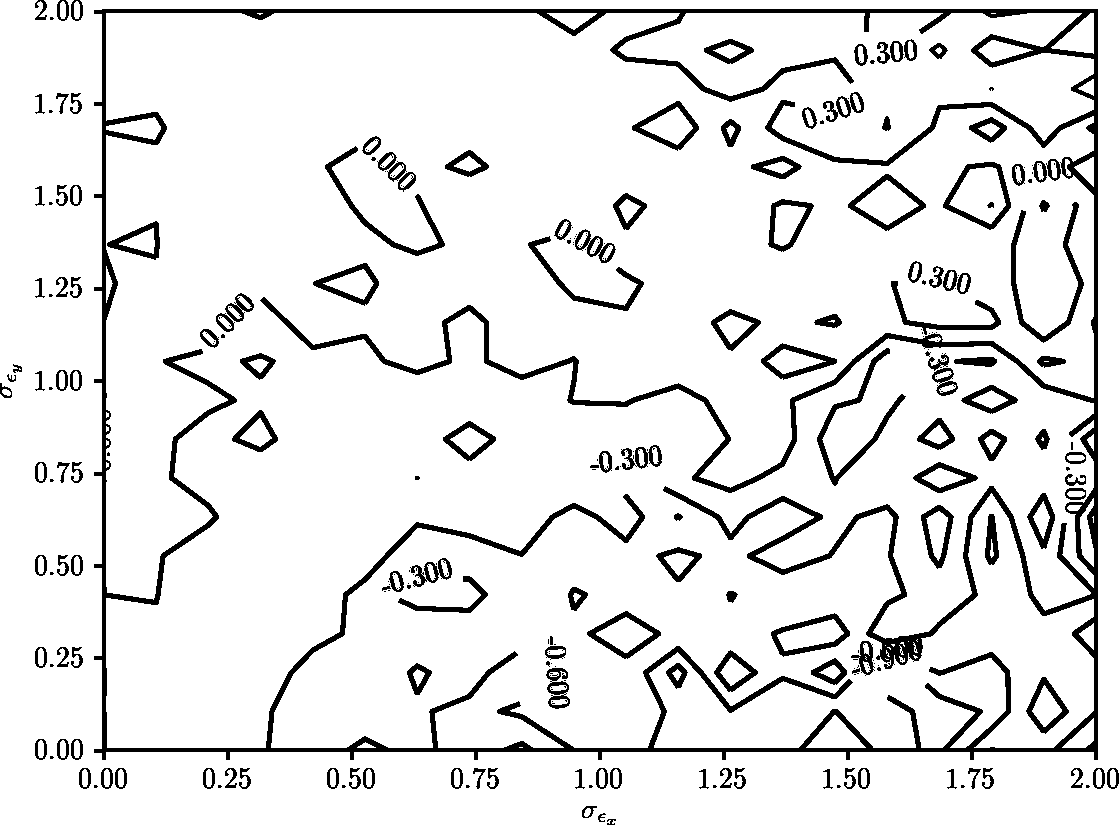
\includegraphics[width=135mm]{fig/nonlinear/quadratic/alpha-5_beta-1.png}
    \caption{\( \theta_1 = 5 \)}\label{fig:comparison_nonlinear_quadratic_alpha-5_beta-1}
  \end{subfigure}

  \vspace{\baselineskip}
  \caption{
    Точность оценивания параметров \\
    параболической модели при \( \theta_2 = 1 \)
  }\label{fig:comparison_nonlinear_quadratic_beta-1}
\end{figure}




\subsection{Кубическая функция регрессии}

\subsection{Экспоненциальная функция регрессии}

\subsection{Синусоидальная функция регрессии}

Эмпирические выводы о точности.